\documentclass[letterpaper,11pt]{article}
\oddsidemargin -1.0cm \textwidth 17.5cm

\usepackage[utf8]{inputenc}
\usepackage[activeacute,spanish, es-lcroman]{babel}
\decimalpoint
\usepackage{amsfonts,setspace}
\usepackage{amsmath}
\usepackage{amssymb, amsmath, amsthm}
\usepackage{comment}
\usepackage{float}
\usepackage{amssymb}
\usepackage{dsfont}
\usepackage{anysize}
\usepackage{multicol}
\usepackage{enumerate}
\usepackage{graphicx}
\usepackage[left=1.5cm,top=2cm,right=1.5cm, bottom=1.7cm]{geometry}
\setlength\headheight{1.5em} 
\usepackage{fancyhdr}
\usepackage{multicol}
\usepackage{hyperref}
\usepackage{wrapfig}
\usepackage{subcaption}
\usepackage{siunitx}
\usepackage{cancel}
\usepackage{mdwlist}
\usepackage{svg}
\usepackage{tcolorbox}
\pagestyle{fancy}
\fancyhf{}
\renewcommand{\labelenumi}{\normalsize\bfseries P\arabic{enumi}.}
\renewcommand{\labelenumii}{\normalsize\bfseries (\alph{enumii})}
\renewcommand{\labelenumiii}{\normalsize\bfseries \roman{enumiii})}


\begin{document}

\fancyhead[L]{\itshape{Facultad de Ciencias F\'isicas y Matem\'aticas}}
\fancyhead[R]{\itshape{Universidad de Chile}}

\begin{minipage}{11.5cm}
    \begin{flushleft}
        \hspace*{-0.6cm}\textbf{FI1000-1 Introducción a la Física Clásica}\\
        \hspace*{-0.6cm}\textbf{Profesora:} Jocelyn Dunstan\\
        \hspace*{-0.6cm}\textbf{Auxiliar:} Alejandro Silva\\
        \hspace*{-0.6cm}\textbf{Ayudantes:} Macarena Muñoz \& Catalina Vargas\\
    \end{flushleft}
\end{minipage}

\begin{picture}(2,3)
    \svgpath{../}  % descomentar si se agrega a carpeta "auxiliares"/"ejercicios"
    \put(366, 10){\includesvg[scale=0.31]{img/dfi.svg}}
\end{picture}

\begin{center}
	\LARGE\textbf{Auxiliar \#10}\\
	\Large{Momento Lineal y Centro de Masa}
\end{center}

\vspace{-1cm}
\begin{enumerate}\setlength{\itemsep}{0.4cm}

\rfoot[]{pág. \thepage}

\item[]

\item Un objeto de masa $m$ resbala sobre la superficie lisa de una cuña de masa $M$. La cuña reposa sobre una superficie lisa. Inicialmente el objeto se encuentra en reposo a una altura $h$ medida desde el tramo horizontal.

\begin{multicols}{2}
    
    \begin{enumerate}
        \item Calcule las velocidades de la cuña y de la masa $m$ una vez que $m$ ha llegado al tramo horizontal de la cuña y esté desplazándose hacia la derecha.
        
        \item Posteriormente, la masa $m$ choca elásticamente con la parte posterior de la cuña. Calcule la rapidez de $m$ y $M$ después del choque.
    \end{enumerate}
    
    \columnbreak
    
    \begin{figure}[H]
        \centering
        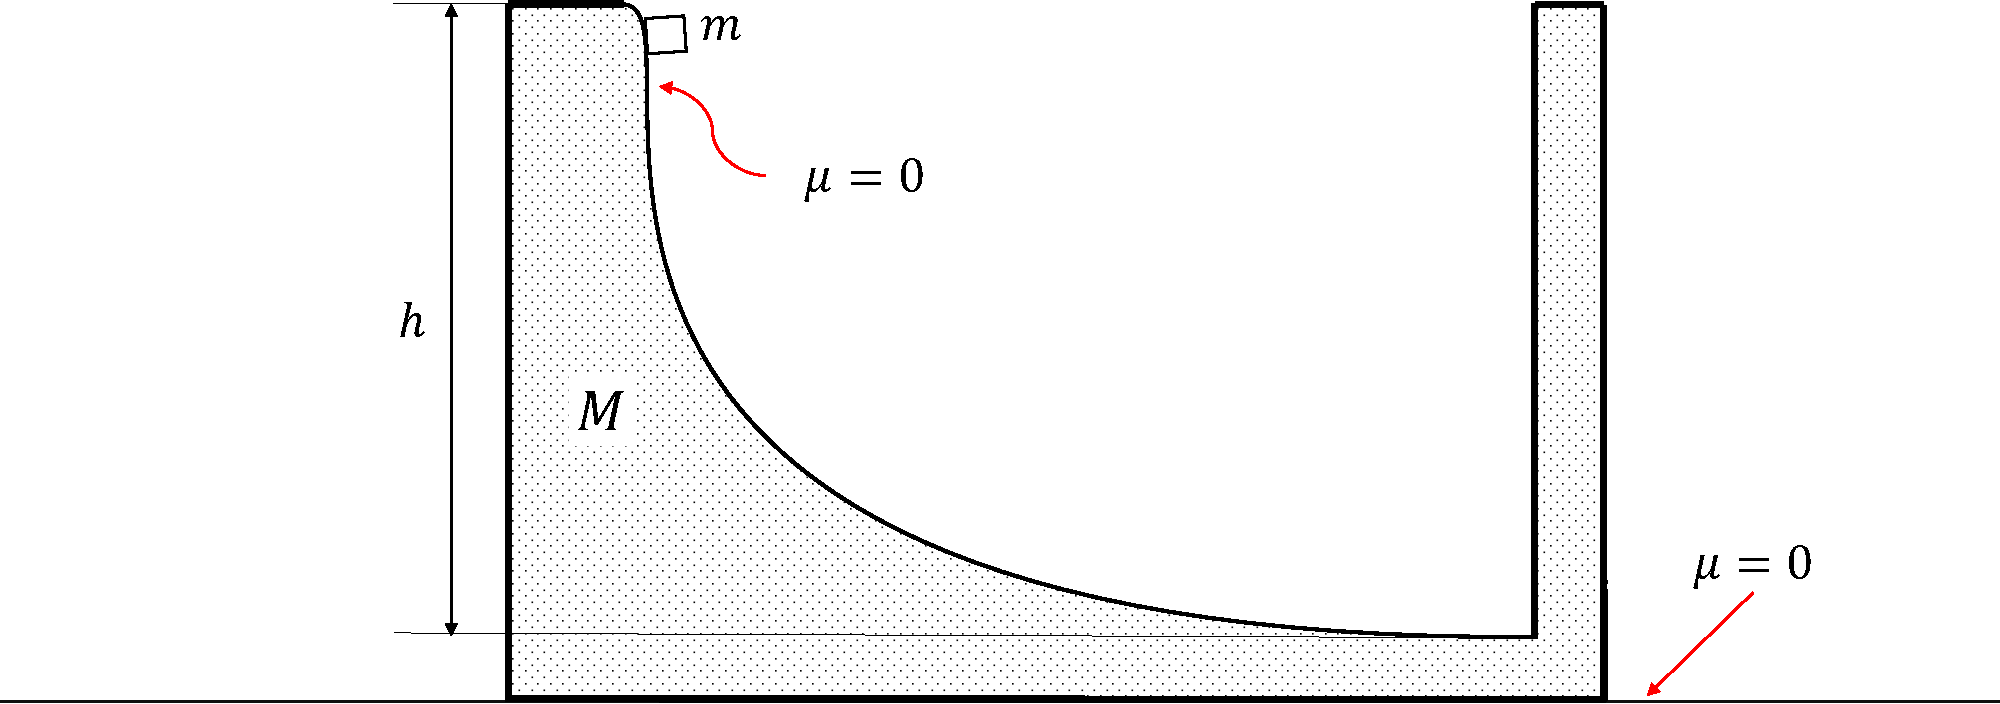
\includegraphics[width=1\linewidth]{2020-1/Imágenes/aux13/cuna.pdf}
    \end{figure}

\end{multicols}

\item Una masa $m$ es soltada desde el punto más alto de un tazón semiesférico de radio $R$, encontrándose en su camino con otra masa de las mismas características, la cual está en reposo en el punto más bajo de aquel, quedando unidas tras el impacto.

\begin{multicols}{2}

    \begin{enumerate}
        \item Despreciando la fricción entre las masas y el tazón, determine la altura máxima alcanzada por el sistema. 
        \item Compare la energía de la situación inicial y final.
    \end{enumerate}
    
    \columnbreak
    
    \begin{figure}[H]
        \centering
        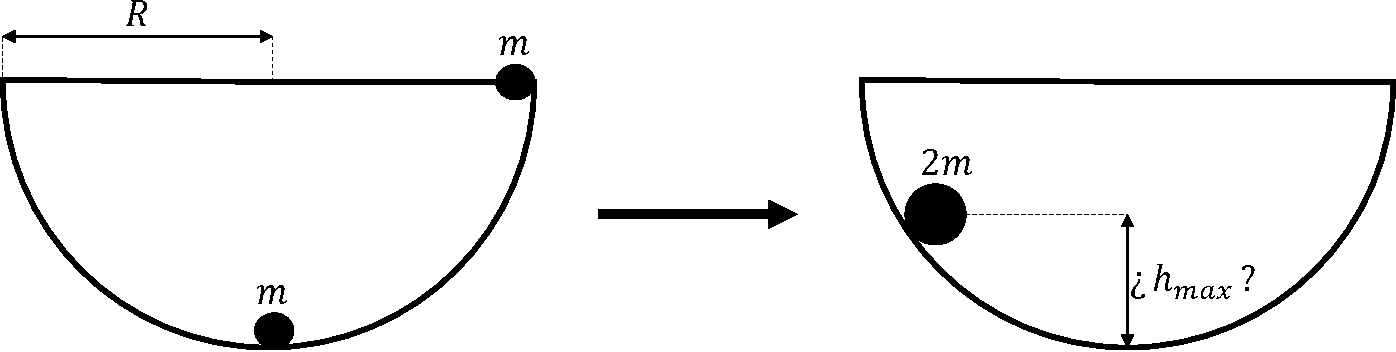
\includegraphics[width=1\linewidth]{2020-1/Imágenes/aux13/sem.pdf}
    \end{figure}
\end{multicols}

\item Romeo y Julieta están sentados en un bote en reposo junto a un muelle. Julieta siente que está muy lejos de Romeo, por lo que decide ir a sentarse a su lado. Para ello camina a una rapidez constante $v$ relativa al agua.

Considere que la masa y la posición con respecto al muelle para Julieta, Romeo y el bote son ($m_j$, $x_j$), ($m_r$, $x_r$), ($m_b$, $x_b$) respectivamente. Además, considere que la distancia inicial que separa a Romeo y Julieta es inicialmente $x_j-x_r=D$.

\begin{multicols}{2}
    \begin{enumerate}
        \item Mientras Julieta está caminando, el bote y Romeo se mueven a rapidez $v'$ en dirección opuesta. Determine la razón $v'/v$
        
        \item Cuando Julieta finalmente se sienta junto a Romeo, ¿qué tan lejos se movió el bote con respecto al muelle?
    \end{enumerate}
    
    \columnbreak
    
    \begin{figure}[H]
        \centering
        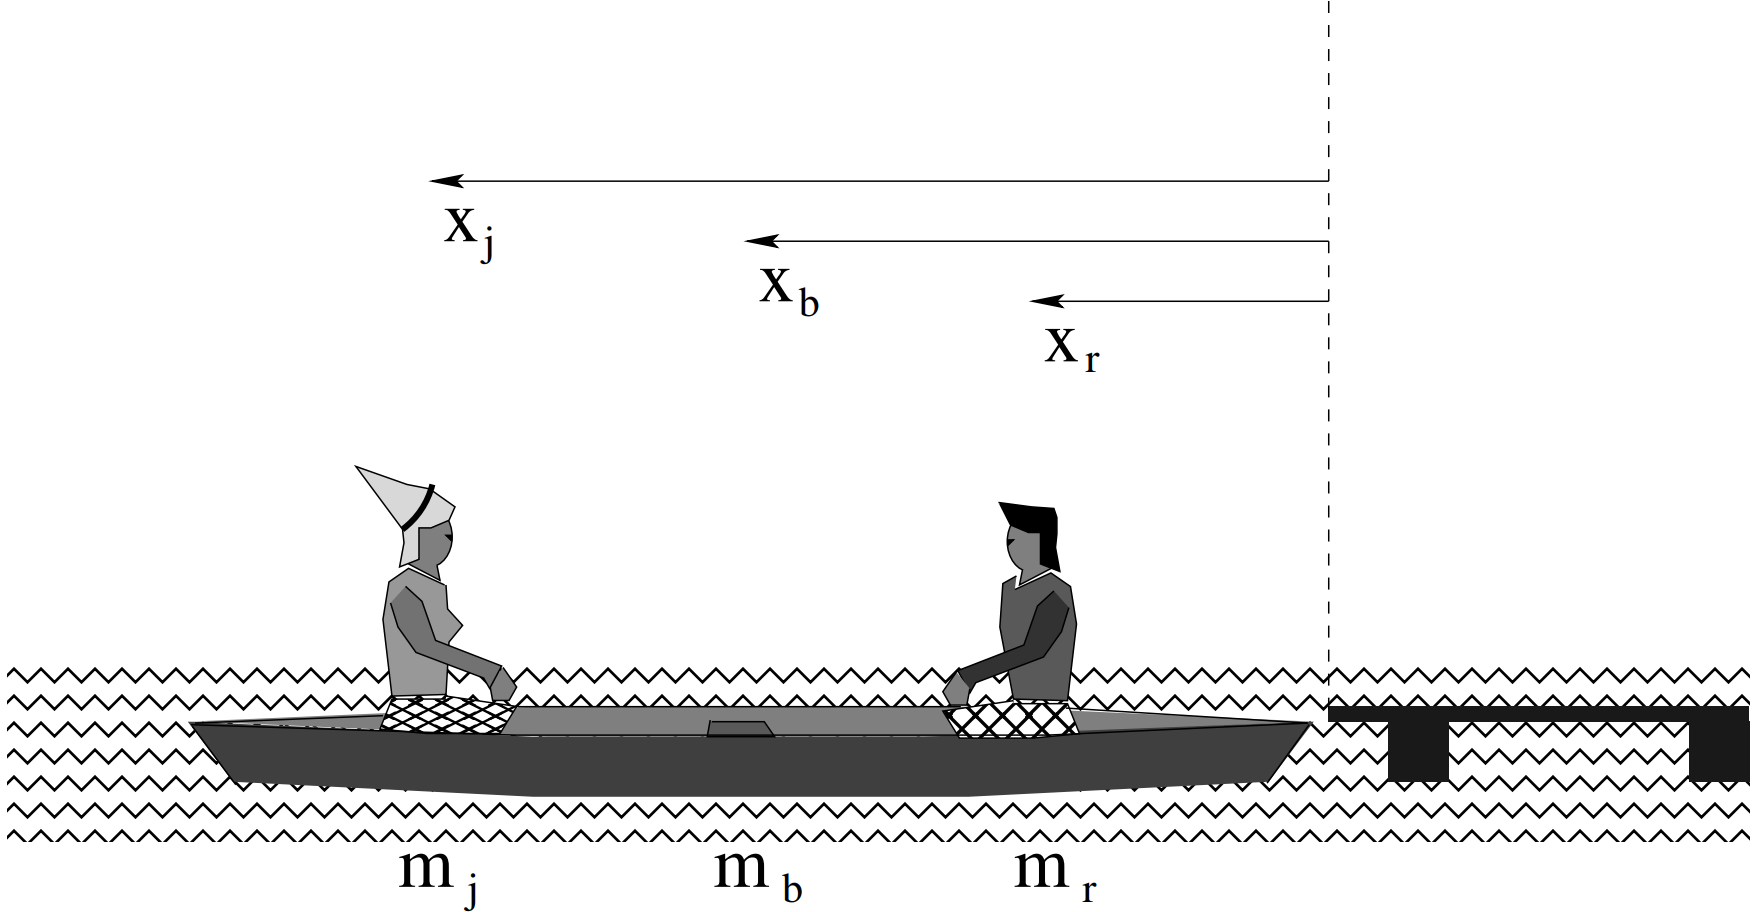
\includegraphics[width=0.7\linewidth]{2021-1/Imagenes/ejercicios/romeo-julieta.PNG}
        %\caption{Romeo y Julieta en el bote}
    \end{figure}

\end{multicols}
\textbf{\textit{Hint:}} Use centro de masa y conservación de momentum, desprecie el roce entre el agua y el bote

\end{enumerate}
\end{document}